
All experiments performed in this \doctype~were running CORE, described in Section \ref{sec:core}, on an Ubuntu 11.04 virtual machine hosted using VMware Fusion on a Mac Air laptop. The experiment emulates a 10 node wireless networking mobile scenario, which consists of 9 consumers (nodes that want to discover a particular service) and 1 producer (a node that wants to advertise a service for use by others).   The mobility patterns for this scenario were generated using an ns-2 mobility pattern generator and then imported into CORE using its inbuilt ns-2 mobile script importer. The emulation runs for 250 seconds and for mobility purposes, the nodes where split into two distinct groups with 5 nodes per group: the first group containing consumers 1-4 and the producer; and the second containing consumers 5-9 inclusively. A screenshot from the CORE GUI representation of this scenario is provide in Figure \ref{indi:fig:core}. The mobile network has a range of 200 meters and a bandwidth of 54 MHz and the entire surface for the emulation covered a surface of  330,000 square meters (600 x 550) with a maximum speed of each node being 20 meters per second. The two clusters of 5 nodes fragment and coalesce around every 30 seconds and therefore there are 4 fragmentations, where the two groups go out of range from each other, during the entirety of the emulation.  This is discussed further in the next section.

\begin{figure}[h!]
\centering
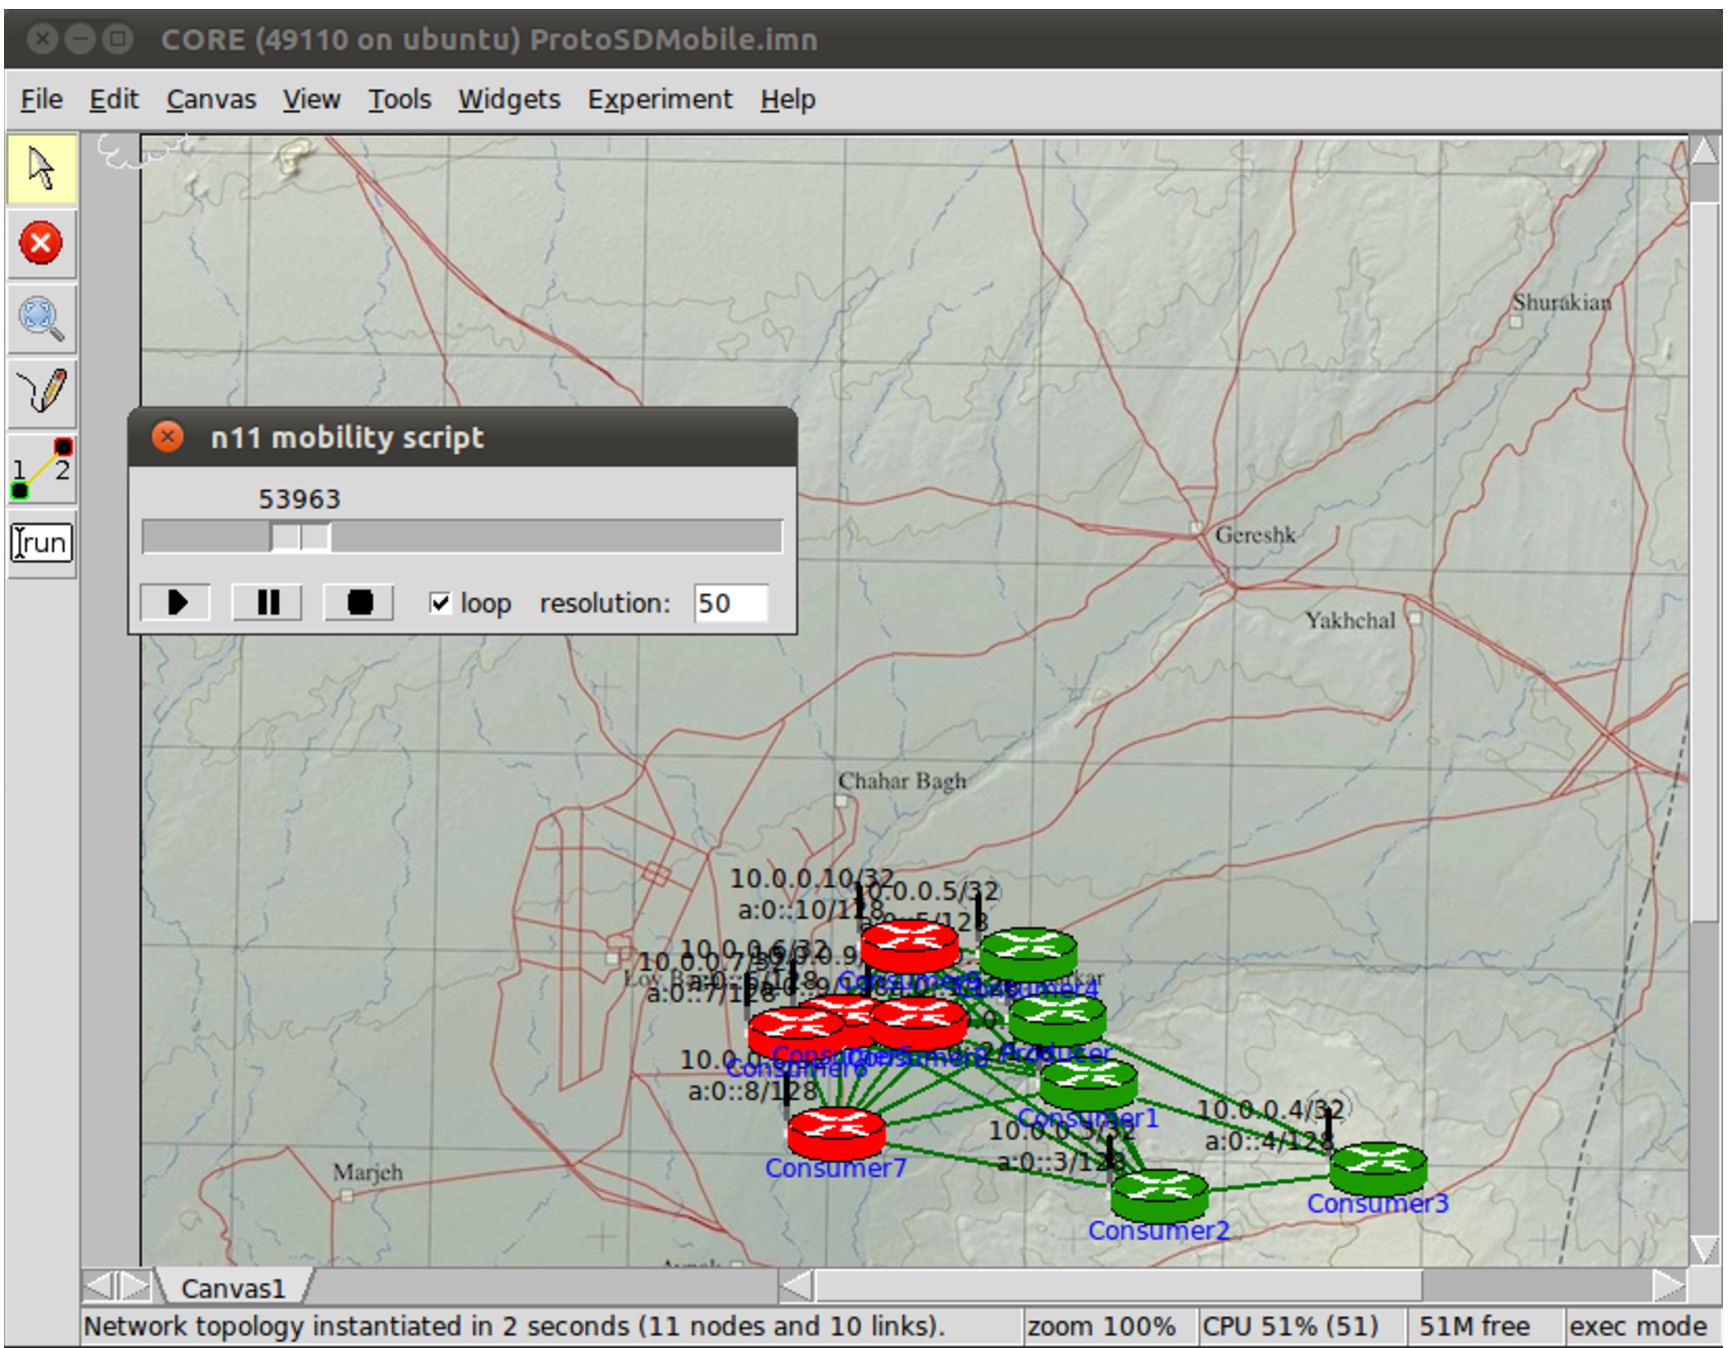
\includegraphics[scale=0.45]{COREEmulation.pdf}
\caption{The running CORE Emulation showing 9 clients and one service running INDI} 
\label{indi:fig:core}
\end{figure}


\subsection{Data Collection}

To collect data from the live emulation experiments, we implemented a distributed file-based event mechanism that gathers information about the low-level packets alongside the higher-level discovery events for each CORE node in a consistent fashion and common format.  Data is collected using one line per event and stored as Comma Separated Values (CSV) for quick-look analysis in Excel and convenient post processing using Java and bash scripts. The CSV files from all CORE nodes are collected in ``tmp/protosd-current'' and time is synchronized across all nodes, which is triggered by the pressing of ``Play''  for initialing the mobility pattern in CORE. This ensures the timing consistency between multiple runs. We record three levels of events:

\begin{description}
\item [At the Packet Level: ] Packet level events are measured using a Java ``tcpdump'' unix process on every core node that records all packets transmitted on the mDNS multicast address (224.0.0.251) on ``eth0'', which is the wireless interface on each CORE node on the emulation.    Packet events store the core node the packet was measured on, the message identifier and its length (in bytes).   The packet level events are used to record the traffic across the course of the emulation in order to construct traffic histograms showing the traffic  at each time-step of the experiment. 

\item [At the Discovery Level: ] Discovery level events record the arrival and departure of services during the course of the emulation.  Service events are recorded from a service producer (when an advert is advertised and removed) and from a consumer (when an advert is resolved and removed)

\item [Multicast Pings: ] In order to automatically detect the mobility pattern during the course of the emulation, we first observe (as a separate run) multicast ping events.  The ``multicast ping'' does not follow the ping protocol but offers a similar level of functionality by sending out packets that can be used to detect whether a server is reachable or not at any given point of time.  In the case of multicast and the one-to-many relationship, we send a multicast message from the producer node to the mDNS multicast address.  All consumers join this multicast group and listen for responses.  
\end{description}


\begin{figure}
\centering
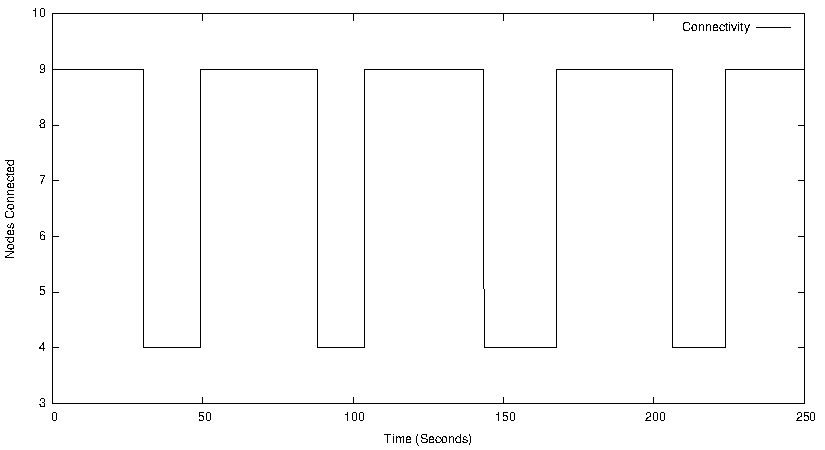
\includegraphics[scale=1.0]{indi10ping-distribution.pdf}
\caption{The connectivity of the two groups of nodes during the course of the 250 second emulation.  The nodes fluctuate between 9
consumers and 4 consumers when the two groups split.} 
\label{indi:fig:emulationconnectivity}
\end{figure}

Multicast ping messages are sent out 10 times per second and we record the event as and when they are received by each consumer to record when each consumer is reachable from the producer.  Ping packets contain an identifier (a simple incremental counter from the producer) along with the sender name. The multicast ping events provide us with a 100 millisecond connectivity matrix for the entire duration of the emulation, which is extremely important, as it allows us to calculate a theoretical limit for the optimal success rates that should be achievable by the service discovery systems.  The result of the ping events can be seen in detail in Figure \ref{indi:fig:emulationconnectivity} for the mobility pattern we used in the emulations.  Multicast ping events are used to generate a histogram that shows the number of consumers that are ``connected''\footnote{The term connected here simply means that a consumer node should be able to receive multicast packets from the producer - it does not imply any protocol-specific usages of this term e.g. TCP.} to the producer at a particular point in time. Therefore, Figure \ref{indi:fig:emulationconnectivity} shows that the number of consumers that are within a multi-hop reachable path of the producer fluctuates between 9 and 4 nodes at the times shown by the X axis of this figure.   This reflects the two distinct groups and the points in the graph where only 4 nodes are connected represents a fragmentation of the two groups.  Therefore, there are 8 transitions during the emulation where the two groups of nodes fragment and then rejoin.   

\subsection{Service Advertisements and Qualitative and Quantitative Metrics}

To measure the responsiveness of the service discovery system for detecting the arrival and departure of services in the face of network fragmentation and dynamics, we generate a sequence of finite-length service advertisements during the course of the emulation.  The adverts are sequentially numbered in chronological order and are named  according to the discovery system that is being used for a particular test (e.g. INDI or mDNS).   For terminology, each advert ``arrives'' in the network when it is advertised and ``departs'' from the network when that service advertisement is removed.    Services are sequenced according to a Poisson distribution and split into three sets with a mean interval of 10, 20 and 30 seconds.  When one advert is advertised the previous advert is simultaneously removed.  

\begin{figure}
\centering
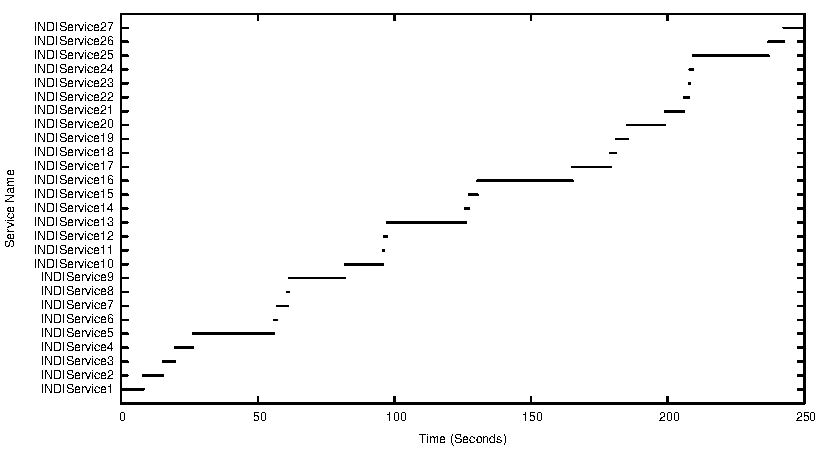
\includegraphics[scale=1.0]{indi10advert-distribution.pdf}
\caption{Shows the time and duration (x axis) that each of the named services (y axis) are advertised for during the emulation.} 
\label{indi:fig:poisson-10-adverts}
\end{figure}

A pictorial representation of the time and duration of services advertised in an emulation, with a Poisson mean interval of 10 seconds, is provided in Figure \ref{indi:fig:poisson-10-adverts}. This diagram shows the emulation time (in seconds) on the x-axis and the name of each service advertised, sequenced by service name and hence arrival time, on the y axis.  In this particular emulation therefore, there are 27 service advertisements during the 250 second emulation, which exhibit Poisson behavior with respect to the time duration they are advertise for.   

In a Poisson exponential probability distribution, the time interval from the current time to the occurrence of the next event does not depending upon the time of occurrence of the last event. This provides a somewhat realistic distribution for modeling real-world random events, such as the arrival of service advertisements in a number of application scenarios. For the same reason, Poisson is often used to model customer arrivals that trigger requests for stress testing web servers.

\begin{figure}
\centering
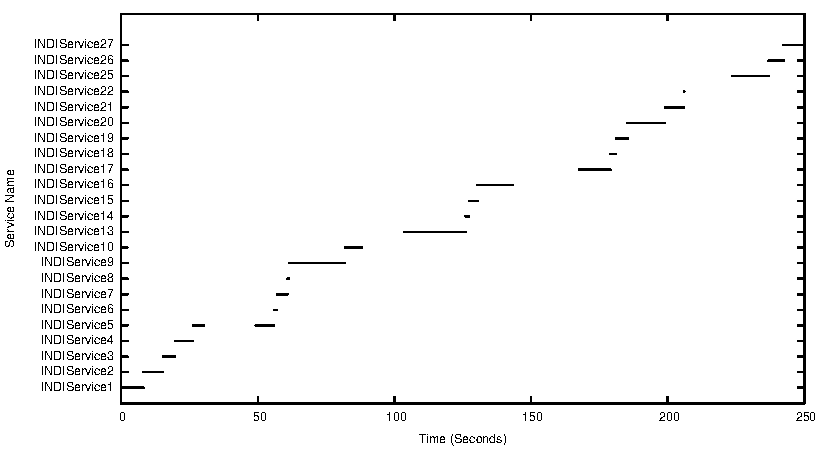
\includegraphics[scale=1.0]{indi10advert-distribution-fragmented.pdf}
\caption{Shows the time and duration (x axis) that each of the named services (y axis) are available for to the fragmented nodes during the emulation.} 
\label{indi:fig:poisson-10-adverts-frag}
\end{figure}


Figure \ref{indi:fig:poisson-10-adverts}  shows the service view from the producer side (server side), which although is also consistent with the permanently connected Consumers 1-4, does not show the consumer view for Consumers 5-9 -- the group of consumers that get fragmented according to the distribution shown in Figure \ref{indi:fig:emulationconnectivity}.  During times of fragmentation therefore, the possibility of discovering the advertisements becomes even more restricted and if we apply this connectivity matrix to the service distribution, we obtain Figure \ref{indi:fig:poisson-10-adverts-frag} that illustrates the actual availability of services advertisements for nodes 5-9 after the fragmentation has been applied to the network.  As one can see, during the periods of fragmentation several adverts e.g. INDIService11, INDIService12, INDIService23 and INDIService24, are not available to these consumers.   

For analysis, the ping traces that are applied to the Poisson distributed service advertisements provide a unique multidimensional view for each consumer with respect to the underlying network behavior and therefore we should take the following two key issues into account when defining the metrics for such an experiment:

\begin{itemize}
\item  \textbf{Optimal Performance:}  If the fragmentation perspective shown in Figure \ref{indi:fig:poisson-10-adverts-frag} is applied algorithmically when analyzing the data, we can calibrate the results according to the optimal discovery performance a service discovery system ``could'' achieve for each service distribution. Therefore, a score of 100\% should be achievable by a system that meets the design constraints of dynamics of the underlying network.  

\item \textbf{Accurate Service Detection:}   Since service distribution can be calibrated to the underlying network connectivity, we also have an accurate Consumer's view of the both the arrival and departure of services. Therefore, a success metric should take into account both the Service Discovery System's ability to detect the arrival of a service and the ability to detect when it is no longer available.
\end{itemize}

As one can plainly see therefore, simple metrics therefore, such as ``success rate'' for discovery and the ``latency'' taken for the service discovery system to discover a service are insufficient for this experiment. In defining a rigorous scientific process for the evaluation of the results, it is important therefore to provide a model that calibrates the results with the above constraints to accurately get a picture of how optimal the system is.  For example, consider the following scenario: service A is advertised at second 2 of the emulation for 48 seconds.  Consumer1 discovers service A but then gets disconnected at second 4 of the emulation and returns in network view of service A at the 45 second on the emulation.  Clearly, here a service discovery system that states the service is available for the entire 46 seconds cannot be deemed successful because for 41 seconds, the service will be unavailable for use.   

A service discovery system therefore needs to track the services as they come in and out of range to give the consumer the highest accuracy possible to avoid service connection errors. In this \doctype, we use the notion of a ``Quality of Service'' (QoS)\footnote{http://en.wikipedia.org/wiki/Quality\_of\_service} to  define the success metric and then we record the latency of both the detection of the arrival and departure of a service.  

QoS is generally used in the context of networking and communication technologies and its goal is to (contractually) mitigate and eliminate unwanted impairments that impact the quality of voice, data and multimedia communications. Therefore, by applying a QoS metric to our service discovery systems, we are forcing a contractual commitment adhering to a certain level of service performance, robustness and reliability. This is in contrast to service discovery systems that happen to delivered on a �best effort basis�  i.e. without QoS guarantees. Therefore, the resulting QoS would naturally lead to a high quality of experience (QoE\footnote{http://en.wikipedia.org/wiki/Quality\_of\_experience}) for a user that wishes to use a particular service. This approach leads to the use of the following two parameters that control the QoS:

\begin{description}
\item[1. Service Discovery Detection for Service Arrival $SDD_{a}$:]   is a constant used to specify the maximum allowable number of seconds for the detection of the arrival of a service to the network.   
\item[2. Service Discovery Detection for Service Departure $SDD_{d}$:]   is a constant  is used to specify the maximum allowable number of seconds for the detection of the departure of a service from the network.    
\end{description}

\noindent and then the \textbf{Success Rate ($SR$)}  is a boolean (true or false) variable that is true if a service is discovered within the defined QoS,  specified below:


\begin{equation}\label{qos}
QoS \equiv (L_a < SDD_a) \wedge (L_d<SDD_d) 
\end {equation} 

where:

\begin{equation}\label{discovery-latency}
L_a= \abs{(D_a - A_a)} 
\end {equation} 

\begin{equation}\label{leaving-latency}
L_d= \abs{(D_d - A_d)} 
\end {equation} 

\noindent and

\begin{itemize}
\item \textbf{$A_a$} is the time the advert was advertised. 
\item \textbf{$A_d$} is the time of the departure of the advert. 
\item \textbf{$D_a$} is the time the discovery system discovered the advert. 
\item \textbf{$D_d$} is the time the discovery system discovered the departure of the advert. 
\end{itemize}

This QoS metric is applied to each of the 9 consumers after the connectivity matrix has been applied, in order to obtain an accurate percentage for the ``optimal performance'' a service discovery system should be capable of achieving for a particular set of services during the emulation. We believe this represents an accurate test for each system.

\normalsize